\documentclass[12pt]{article}

%preamble%%%%%%%%%%%%%%%%%%%%%%%%%%%%%%%%%%%%%%%
%\usepackage{ctex}
\usepackage{geometry}
\geometry{left=1in,right=0.75in,top=1in,bottom=1in}
\usepackage{makeidx}
\makeindex

\bibliographystyle{plain}
\usepackage{algorithm}
\usepackage{algpseudocode}
\usepackage{newtxtext}
\usepackage{amsmath,amssymb,amsthm}
\usepackage{newtxmath} % must come after amsXXX
\usepackage[pdftex]{graphicx}
\usepackage{xcolor}
\usepackage{fancyhdr}
\usepackage{appendix}
\usepackage{booktabs}

\lhead{Team \Team}
\rhead{}
\cfoot{}

\newtheorem{theorem}{Theorem}
\newtheorem{corollary}[theorem]{Corollary}
\newtheorem{lemma}[theorem]{Lemma}
\newtheorem{definition}{Definition}[section]

\newcommand{\Problem}{ABCDEF}
\newcommand{\Team}{2400609}

\renewcommand\appendixtocname{Appendix}
%%%%%%%%%%%%%%%%%%%%%%%%%%%%%%%%%%%%%%%%%%%

\begin{document}

\graphicspath{{.}}  % Place your graphic files in the same directory as your main document
\DeclareGraphicsExtensions{.pdf, .jpg, .tif, .png}

%Summary%%%%%%%%%%%%%%%%%%%%%%%%%%%%%
\thispagestyle{empty}
\vspace*{-16ex}
\centerline{\begin{tabular}{*3{c}}
	\parbox[t]{0.3\linewidth}{\begin{center}\textbf{Problem Chosen}\\ \Large \textcolor{red}{\Problem}\end{center}}
	& \parbox[t]{0.3\linewidth}{\begin{center}\textbf{2024\\ MCM/ICM\\ Summary Sheet}\end{center}}
	& \parbox[t]{0.3\linewidth}{\begin{center}\textbf{Team Control Number}\\ \Large \textcolor{red}{\Team}\end{center}}	\\
	\hline
\end{tabular}}

\begin{center}
	\Large \textbf{Shortest Path Algorithms:~Taxonomy and Advance in Research}
\end{center}

As for problem 1,  in order to accurately capture the effective information in the data 
set, we take a series of data processing methods... After that, we select potential influencing
factors and establish Analytic Hierarchy Process (AHP) model to make a preliminary analysis of the influencing
factors and calculate specific parameters for each factor. We find that the biggest factor is 
score difference. Apart from that ,whether scored in the last point, running distance, unforced error and fast win
will also positively or negatively influence the momentum to a comparatively large extent. The above conclusion is verified
in our later models.\\

In problem 2, we believe that momentum will affect the future scores of the match. So to answer the coach's question, 
we first perform autocorrelation test on momentum, and we find that it has strong first-oredr autocorrelation. Then we quantify 
the future scores and then determine the correlation of momentum the scores in the future, they are highly correlated.\\

Problem 3 is devided into 3 parts. To predict the swings in the match , we establish model based on Gated Recurrent Unit(GRU) algorithm.
We process data in problem 1 and add more features. We define the swings and use previous information to predict future.
Then compared to the result in problem 1, our accuracy is ....\\

To identify the most related factors, we use a novel argorithm called Permutation Feature Importance argorithm, 
it can determine the importance of features by calculating their prediction error after permutation. We find that ....\\

As for the ideas for specific atheletes, we use previous model on their matches to identify their feature importance.
We find that different atheletes have different features in their match.\\

Problem 4\\

Key words: AHP, correlation analysis, GRU, Permutation Feature Importance

Indroduction\\
Tennis more than any other sport, is a game of momentum. 
The absence of a clock to do the dirty work of finishing off an opponent, 
and a scoring system basedon units used, makes the flow of the match much more important than any 
lead that has been established.--Chuck Kriese\\

problem3

Using the above argorithm, we sort FI and normalize them, then we plot the figure:

\begin{figure}[H]
    \centering
    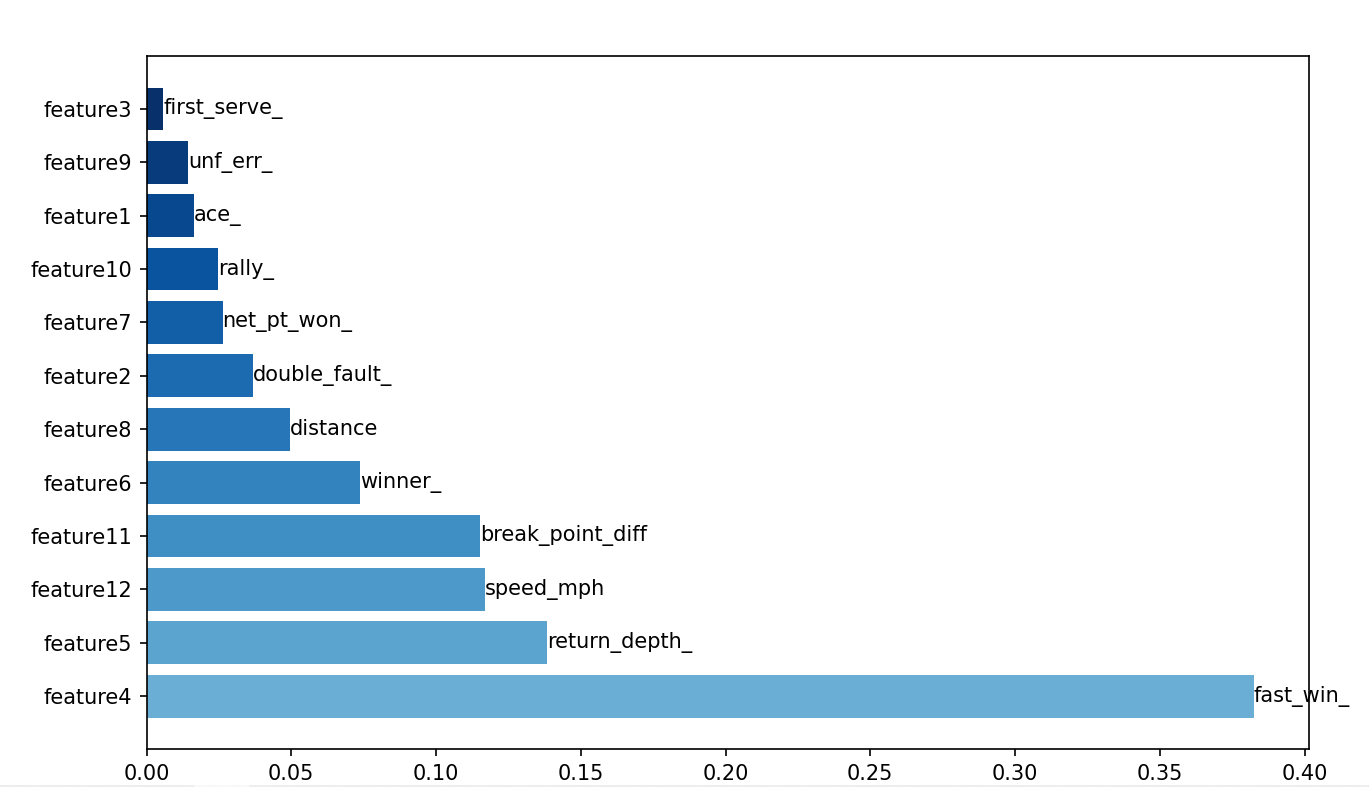
\includegraphics[scale=0.6]{mainmatter/imgs/8.png}
    \caption{feature importance}
\end{figure}

We can see that the most important feature is fast win(rally count < 3 and wins the point),
Because this time we only consider skill factors.this is related to our previous work,
%table of contents%%%%%%%%%%%%%%%%%%%
\tableofcontents 

%main matter%%%%%%%%%%%%%%%%%%%%%%%%%
\newpage
\setcounter{page}{1}
\rhead{Page \thepage\ }

\section{Introduction}

test

\subsection{Overview}

test

\subsection{Restatement of the Problem}

\paragraph{First Problem}

Momentum is “strength or force gained by motion or by a series of 
events.”It directly shows the player's current performance.
To assess the players' performance, it is crucial to have a clear understanding of ``momentum.'' 
We will focus on the following tasks: 
\begin{itemize}
    \item determine the influencing factors of ``momentum''
    \item Quantify the variations in ``momentum'' .
    \item Visualize the process of ``momentum'' changes.
\end{itemize}

\paragraph{Second Problem}

``momentum's role in the match'' means the level of momentum affects the future scores of the match.
The coach may subscribe to the idea that each point is an independent event and governed by probability.
In this view, consecutive success and momentum changes (swings) are seen as more random than influenced by previous events.
To judge this autocorrelation and to use our model, we 

\begin{itemize}
    \item perform autocorrelation test on momentum
    \item perform correlation test between current momentum and future scores.
\end{itemize}



\subsection{Assumptions}

To simplify the problem, we made the following assumptions:

\begin{itemize}
    \item \textbf{Assumption 1:} The \verb|px_unf_err| column of the data only counts those unforced errors that occurred when the player was hitting in baseline.\\
    \textbf{Justification:} Usually when a player is at net, the point will end in a few strikes, and there's little probability that the player will hit an unforced error within that few strikes. What's more, the \verb|px_net_point| and \verb|px_net_point_won| columns of the data can predominantly reflect the player's ability at net, therefore reducing the impact of counting the unforced errors while at net.
    
    \item \textbf{Assumption 2:} The current performance on a certain aspect of a player can be reflected by the player's 3 latest shots of that aspect.\\
    E.g. $P_{ace}$ can be reflected by the proportion of aces in the 3 latest \textbf{serves} of the player, $P_{win}$ can be reflected by the proportion of winners in the 3 latest \textbf{shots} of the player, $rd$ can be reflected by the return depth of the 3 latest \textbf{returns} of the player, etc. \\
    \textbf{Justification:} The current performance of a player consists of the average performance and the status of the player at the moment, which can be comprehensively reflected in the player's performance on recent shots. For convenience, we specified that the 3 latest shots can reflect the player's current performance.
\end{itemize}

\subsection{Our Work}

\begin{itemize}
    \item develop a model to 
\end{itemize}

\section{Notations and asssumptions}
\subsection{Notations}

test

\subsection{Assumptions}

test

\section{... Model}
\begin{definition}
    Niche width is the range of resources that a species can use.
\end{definition}
Niche width is an indicator \cite{Alice13}

\subsection{Model Overview}

\begin{algorithm}
    \caption{An algorithm with caption}\label{alg:cap}
    \begin{algorithmic}
    \Require $n \geq 0$
    \Ensure $y = x^n$
    \State $y \gets 1$
    \State $X \gets x$
    \State $N \gets n$
    \While{$N \neq 0$}
    \If{$N$ is even}
        \State $X \gets X \times X$
        \State $N \gets \frac{N}{2}$  \Comment{This is a comment}
    \ElsIf{$N$ is odd}
        \State $y \gets y \times X$
        \State $N \gets N - 1$
    \EndIf
    \EndWhile
    \end{algorithmic}
\end{algorithm}

\section{Robustness Analysis}

\subsection{Generalization ability}

Now, we have finished Problem 4.

\subsection{Parameters Sensitivity Analysis}

\section{Strength and Weaknesses}

\subsection{Strengths}

\begin{enumerate}
    \item {\bf Visualization in conclusion}: Visualization is used to interpret the result, making it intuitive and concise.
    \item {\bf Proper models chosen}: Two models in problem 1 and problem 3 have similar results of the influencing factors, which makes it more reliable.
    \item {\bf Stable performance}: Our model has stable prediction in different men's matches.
    \item {\bf Classification of different situations}: We evaluate momentum in two different situations, serve and opponent serve.
\end{enumerate}


\subsection{Weaknesses}

\begin{enumerate}
    \item {\bf A little subjective}: In problem 1, AHP is a subjective method to some extent, so although we get desired result similar to problem 3,
    some new completely objective method needs to be carried out.
    \item {\bf Limited ability in predicting other kinds of matches}: The technical indexes are different in other matches, so if we want to predict them, 
    we need to do some modification on our model.
\end{enumerate}

%back matter%%%%%%%%%%%%%%%%%%%%%%%%%
\addcontentsline{toc}{section}{Refences}
\bibliography*{backmatter/papers}

\appendix
Begin your appendix here.
\section{1}
test
\subsection{1}
test
\subsubsection{1}
test
\paragraph{1}
test
\subparagraph{1}
test

\section{report on Use of AI}

\cite{Alice13}

1.

OpenAI ChatGPT (Feb 2,2024 version,ChatGPT3.5)

Query1:  \emph{
    “swings in play and runs of success by one player are random” 
can this sentence to be interpreted as  swings in play and runs of success by one player are independent?
}

Output: \emph{Yes, the sentence "swings in play and runs of success by one player are random" 
can be interpreted as suggesting that swings in play and runs of success by one player are 
independent of each other. In statistical terms, independence means that the occurrence or 
outcome of one event does not influence the occurrence or outcome of another.}

\emph{
In the context of tennis, this would imply that the fluctuations in the dynamics of the match 
(swings in play) and a player's success streaks (runs of success) are not connected or dependent 
on each other. Each event is considered random and not influenced by the occurrence of the other.
}

\end{document}